\section{W-mass}
\label{sec:w-mass}
With the finished calibration, the mass of the W-boson can now be measured. 
In order to determine the W-mass, we use a data set of actual ATLAS data containing $W \rightarrow e\nu$ events,
as well as several simulated data sets also containing $W \rightarrow e\nu$ events. 
There is also a $Z^0 \rightarrow e^+e^-$ data set to check the validity of the previous calibration. Finally there are data sets for QCD- and non-QCD background events.

\subsection{Electron Calibration Verification}

\begin{figure}[H]
    \centering
    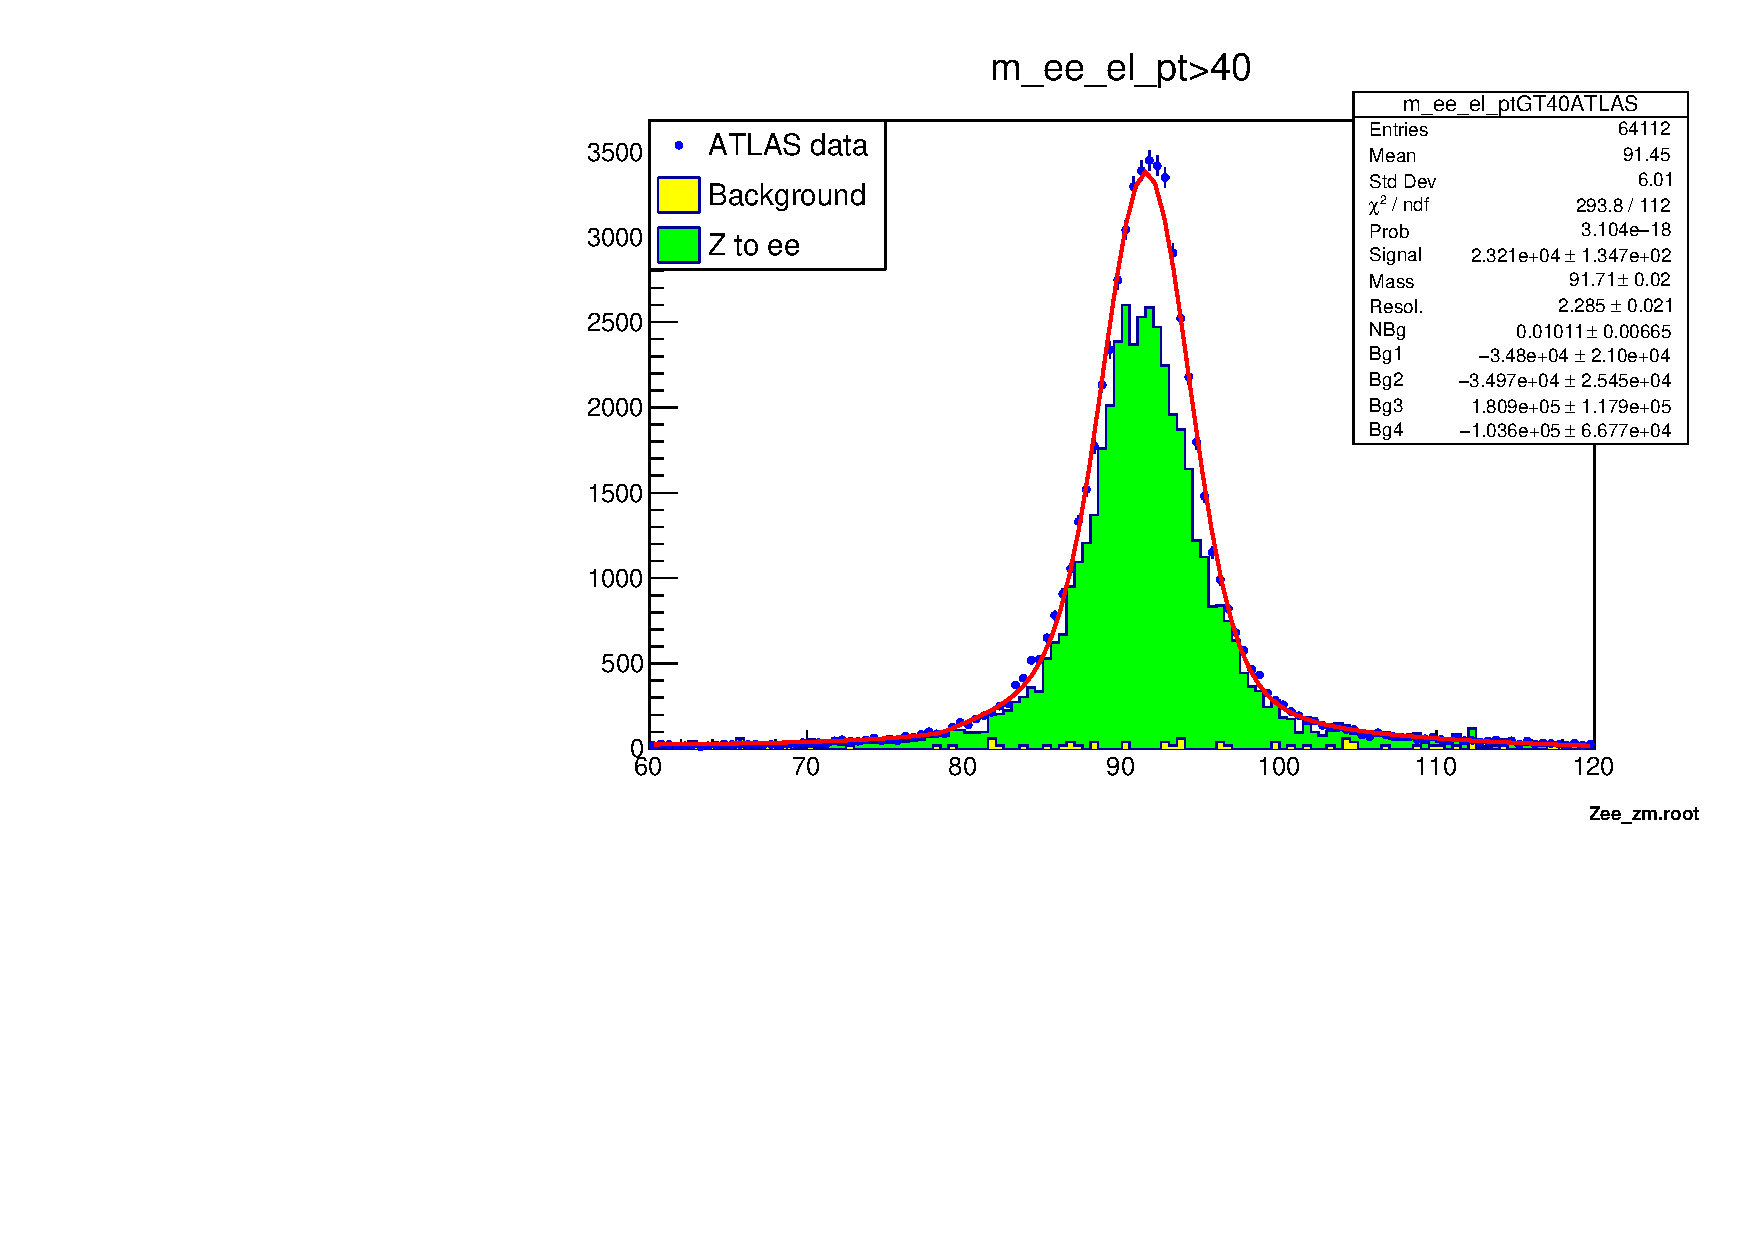
\includegraphics[width=0.6\textwidth]{../W_mass/Z_mass_check_el_pt-cut.pdf}
    \caption{$Z_mass_check_el_pt-cut.pdf$}
    \label{fig:z-mass_check}
\end{figure}
\subsection{QCD scale factor}

\subsection{Cut selection}

\subsection{Gauge curves}

\subsection{W-mass }